\newpage
\setcounter{section}{0}
\renewcommand{\thesection}{\arabic{section}}

\begin{center}
    \Huge
    \textbf{Modul 4}
    
    Konfigurasi VPN(Virtual Private Network) PPTP pada Mikrotik

\end{center}


\section{Pendahuluan}

VPN atau Jaringan Pribadi Virtual (Virtual Private Network) membuat koneksi jaringan privat di
antara beberapa perangkat melalui internet. VPN digunakan untuk mentransmisikan data secara aman
dan anonim melalui jaringan publik. VPN bekerja dengan cara menyembunyikan alamat IP pengguna
dan mengenkripsi data sehingga tidak dapat dibaca oleh siapa pun yang tidak berwenang untuk
menerimanya.

Salah satu service yang biasa digunakan untuk membangun sebuah jaringan VPN adalah Point to
Point Tunnel Protocol (PPTP). Sebuah koneksi PPTP terdiri dari Server dan Client.
Mikrotik RouterOS bisa difungsikan baik sebagai server maupun client atau bahkan diaktifkan
keduanya bersama dalam satu mesin yang sama. Feature ini sudah termasuk dalam package PPP
sehingga anda perlu cek di menu system package apakah paket tersebut sudah ada di router atau
belum. Fungsi PPTP Client juga sudah ada di hampir semua OS, sehingga kita bisa menggunakan
Laptop/PC sebagai PPTP Client.

Biasanya PPTP ini digunakan untuk jaringan yang sudah melewati multihop router (Routed Network).
Jika anda ingin menggunakan PPTP pastikan di Router anda tidak ada rule yang melakukan blocking
terhadap protocol TCP 1723 dan IP Protocol 47/GRE karena service PPTP menggunakan protocol
tersebut.

\section{Tujuan Praktikum}

Mengetahui cara menggunakan dan mengkonfigurasi VPN PPTP pada router mikrotik.

\section{Alat dan Bahan}

Berikut adalah Alat dan Bahan untuk praktikum:

\begin{enumerate}
    \item 2 Cloud Core Router
    \item 3 Kabel UTP (LAN)
    \item 3 Laptop
    \item Software Winbox
\end{enumerate}

\section{Topologi}

berikut adalah topologi yang digunakan :

\begin{center}
    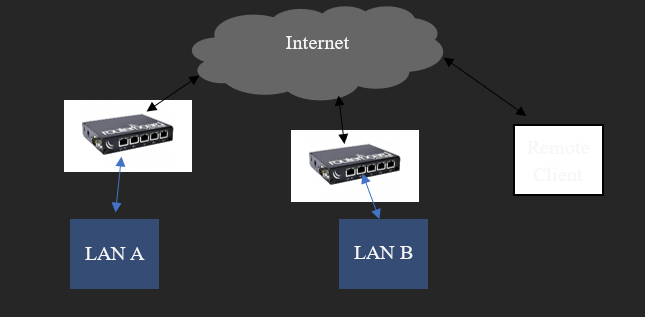
\includegraphics[width=0.7\textwidth]{image/P4/Topologi.png}    
    
    figure.1 Topologi
\end{center}

\section{Langkah Percobaan}
\begin{enumerate}
    \item Sambungkan PC dan router mikrotik sesuai dengan topologi
    \item Matikan firewall di laptop
    \item Masuk ke aplikasi Winbox
    \item Pada bagian Neighbour, check apakah ada IP 0000 identity mikrotik
    \item Reset mikrotik ke 0000
    \item Lalu tekan connect
    
    \begin{center}
        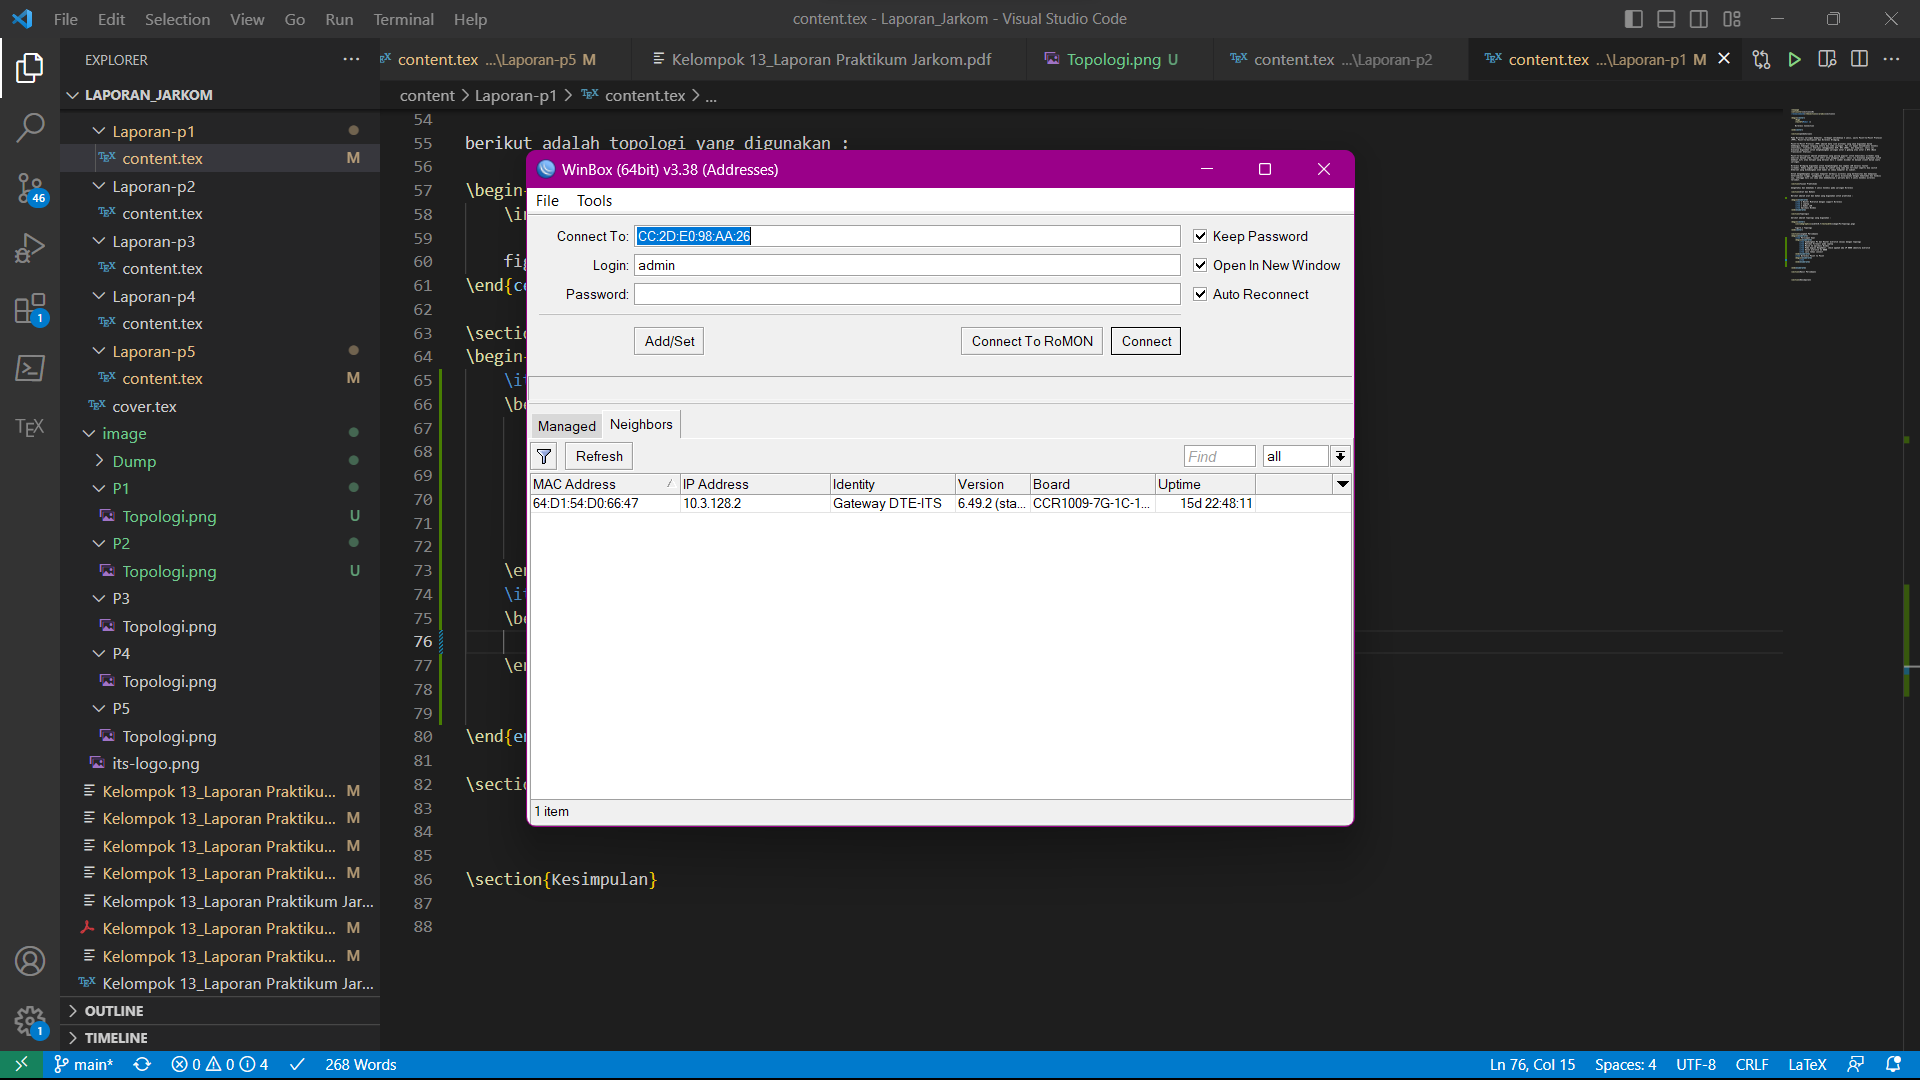
\includegraphics[width=0.7\textwidth]{image/Winbox-interface.png}    
        
        figure.2 WinBox interface
    \end{center}
    
    \item Lakukan konfigurasi DHCP agar dapat terhubung dengan ISP, pilih menu IP \texttt{\text>} DHCP Client \texttt{\text>} (+) \texttt{\text>} Interface : ether 1 (yang terhubung pada ISP)
    \item Kemudian secara otomatis akan didapatkan IP dari ISP
    \item Lalu pilih menu IP \texttt{\text>} Firewall \texttt{\text>} NAT \texttt{\text>} Chain : srcnat, Out. Interface : ether 1
    \item Kemudian pilih menu IP \texttt{\text>} Firewall \texttt{\text>} NAT \texttt{\text>} Action : masquerade
    \item Setelah itu atur routes untuk ether 1 secara static, pilih menu IP \texttt{\text>} Routes \texttt{\text>} (+) \texttt{\text>} Dst Address : 0.0.0.0/0, Gateway : (gateway IP address yang telah diberikan ISP) \texttt{\text>} Apply
    \item Setelah terlihat status “reachable” pada Route List, kemudian atur DNS
    \item Untuk mengaktifkan PPTP server, pilih menu PPP \texttt{\text>} Interface \texttt{\text>} PPTP Server \texttt{\text>} Default Profile : default encryption
    \item Kemudian buatlah secret untuk mengakses server, pilih menu New PPP Secret \texttt{\text>} Profile : default encryption , Local Address : (address PPTP server) , Remote Address : (IP yang akan diberikan ke client)
    
    \begin{center}
        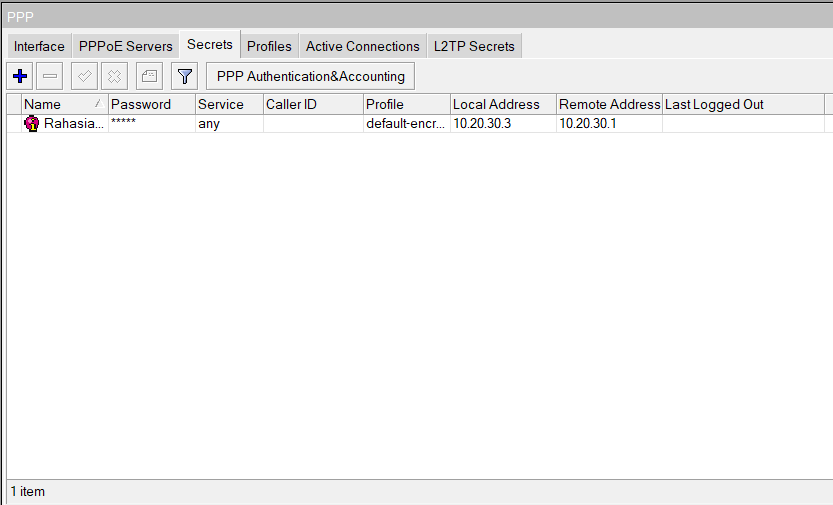
\includegraphics[width=0.7\textwidth]{image/P4/ppp.png}    
        
        figure.3 PPP Server
    \end{center}

    \item Isikan nama dan password, pastikan nama dan password mudah untuk diingat
    \item Lalu lakukan konfigurasi client PPTP, pilih menu PPTP Client \texttt{\text>} New Interface \texttt{\text>} Connect To : (IP public server yang dituju)
    \item Kemudian pada kolom User dan Password, masukkan nama dan password sesuai secret yang sudah dibuat
    \item Setelah itu lakukan static routing, pilih menu New Route \texttt{\text>} Dst. Address : (jaringan local router lawan) , Gateway : (IP PPTP tunnel pada router lawan)
    
    \begin{center}
        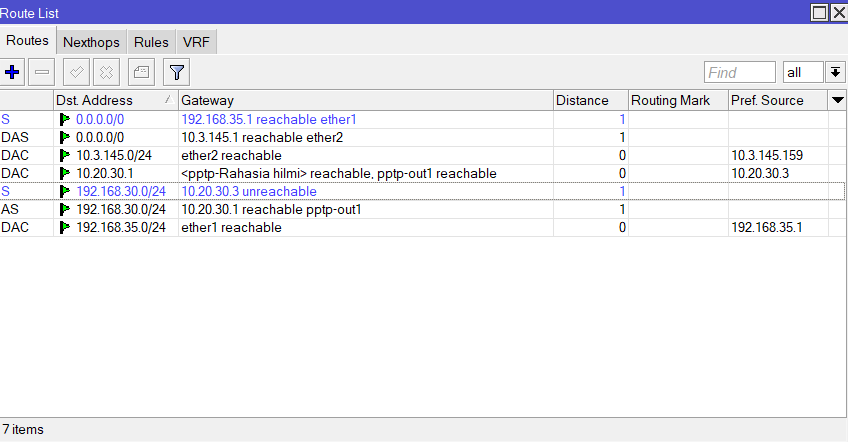
\includegraphics[width=0.7\textwidth]{image/P4/Route-list.png}    
        
        figure.4 Virtual Route List
    \end{center}

    \item Untuk melakukan remote client, perlu dibuat secret baru dengan cara yang sama dengan sebelumnya
    \item Agar remote client dapat terhubung ke server, perlu dilakukan setup connection pada sisi client
    \item Pergi ke setting dan pilih menu Network and Sharing Center \texttt{\text>} Set up new connection or network \texttt{\text>} Connect to a workplace \texttt{\text>} Use My Internet Connection (VPN) \texttt{\text>} Internet address : (IP public server yang dituju) \texttt{\text>} Next
    \item Kemudian masukkan nama dan password sesuai secret yang sudah dibuat untuk remote client
    \begin{center}
        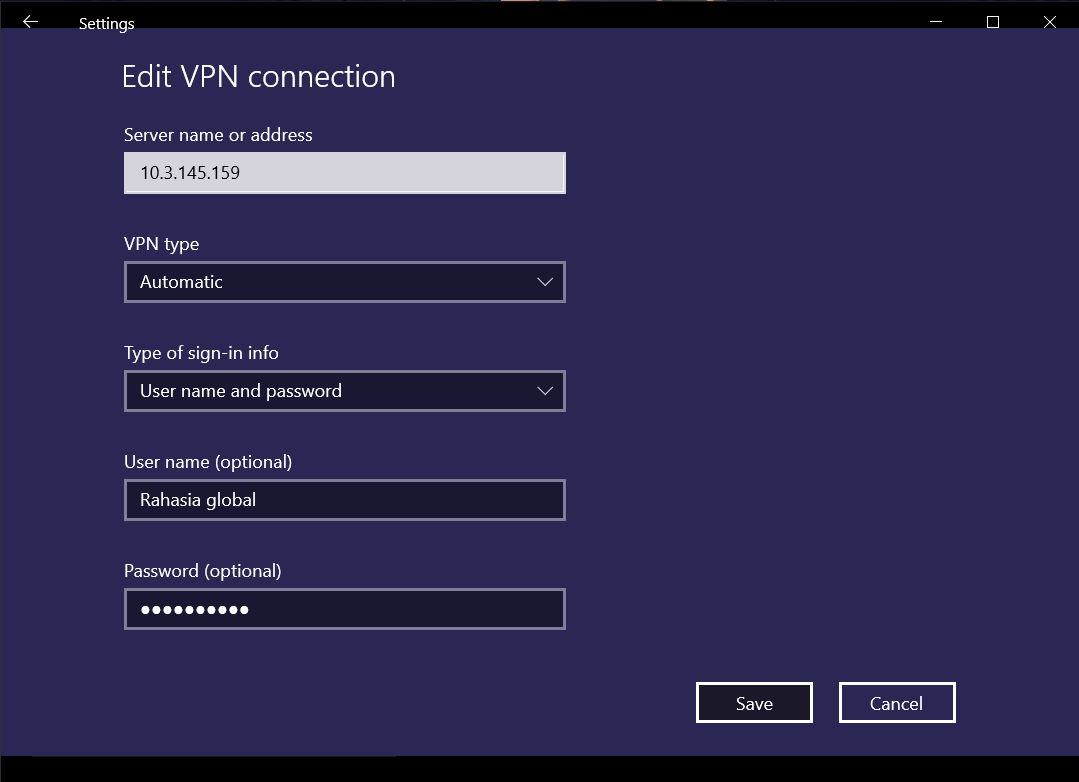
\includegraphics[width=0.7\textwidth]{image/P4/Client-vpn.jpg}    
        
        figure.5 VPN Set up
    \end{center}

\end{enumerate}

\section{Hasil Percobaan}

Router Test
    
\begin{center}
    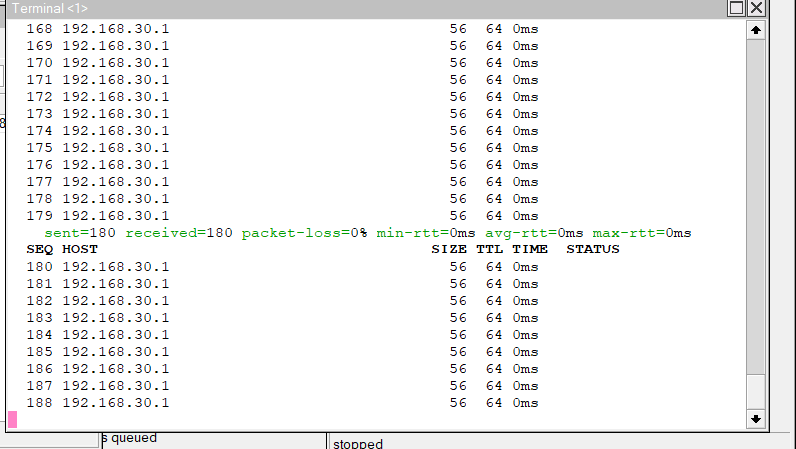
\includegraphics[width=0.7\textwidth]{image/P4/route-test.png}    
    
    figure.6 Route Testing
\end{center}

Client test

\begin{center}
    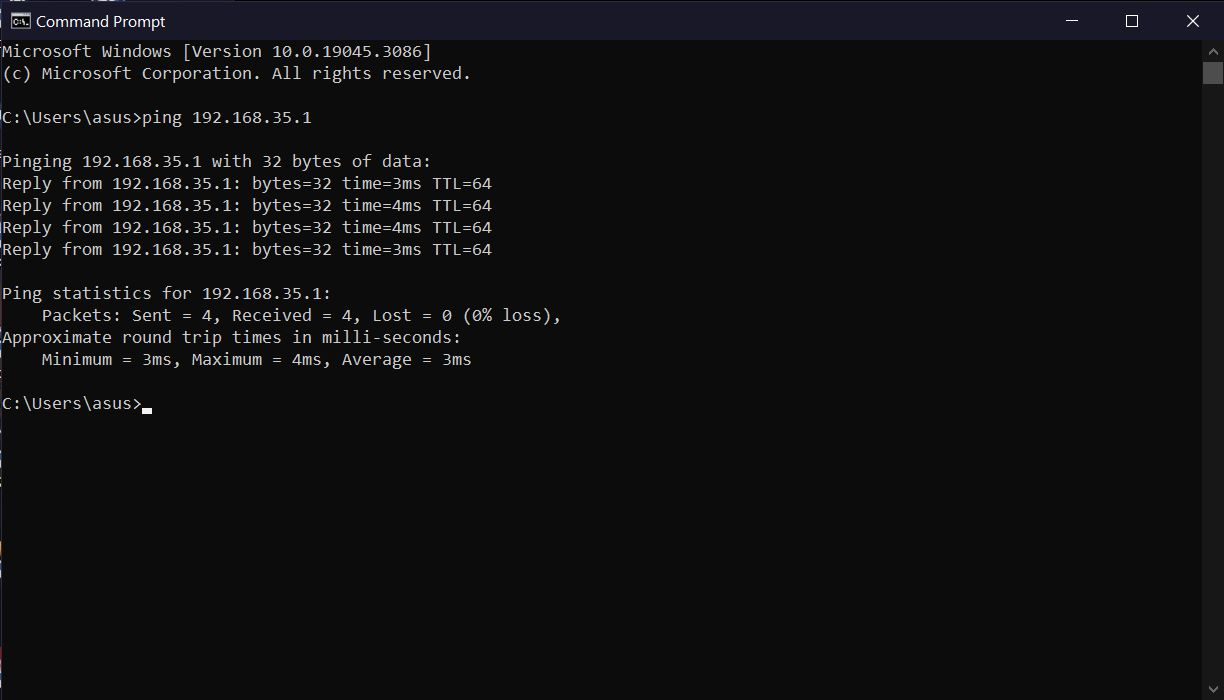
\includegraphics[width=0.7\textwidth]{image/P4/client-test.jpg}    
        
    figure.7 Client Testing
\end{center}

\section{Kesimpulan}

PPTP dapat digunakan untuk membuat suatu Virtual Private Network(VPN)

\section{Tugas modul}

\begin{enumerate}
    \item PPTP memiliki kelemahan yaitu tidak menyediakan mekanisme otentikasi server yang kuat, sehingga rentan terhadap serangan MITM(Man in the Middle). Untuk memitigasi hal ini dapat dilakukan dengan menambahakan enkripsi tambahan, misalnya dengan menggunakan protokol enkripsi seperti L2TP/IPS-\\ec untuk melindungi lalu lintas data yang dikirim melalui koneksi PPTP.

    \item Alternatif protokol VPN yang lebih aman dibandingkan PPTP salah satunya adalah IPSec(Internet Protocol Security). Apabila dibandingkan dengan PPTP, IPSec menggunakan enkripsi yang lebih kuat, protokol otentikasi yang lebih andal, dan sering kali memiliki mekanisme keamanan tambahan yang diperbarui secara teratur.
    
    \item Kelebihan utama yang dimiliki oleh PPTP yaitu kemudahan implementasi. Penggunaan dan pengaturan PPTP lebih sederhana dibandingkan dengan protokol VPN lain yang mungkin memerlukan konfigurasi yang lebih kompleks. Selain itu PPTP juga memiliki kinerja yang cepat karena protokol PPTP dirancang untuk memberikan koneksi yang stabil dan responsive dengan beban yang lebih rendah pada jaringan.
    
    \item Beberapa kekurangan dan batasan penggunaan PPTP sebagai protokol VPN antara lain yaitu kelemahan keamanan, tidak didukung oleh banyak perangkat, tidak dapat melewati firewall yang ketat, dan tidak dapat digunakan di beberapa negara atau jaringan.
    
    \item Langkah-langkah untuk mendiagnosis masalah dalam mengkonfigurasi VPN PPTP diantaranya yaitu dengan memeriksa pengaturan server VPN, memeriksa pengaturan klien VPN, memeriksa koneksi jaringan, memeriksa firewall dan perangkat jaringan, memeriksa log dan pesan kesalahan, mencoba koneksi dari lokasi lain, atau dengan memperbarui perangkat lunak.
    
    \item Solusi alternatif PPTP diantaranya yaitu dengan menggunakan protokol VPN berbasis SSL(Secure Socket Layer)/TLS(Transport Layer Security) maupun VPN berbasis SSH(Secure Shell). Dan apabila masalah masih tidak dapat diatasi, pertimbangkan menggunakan layanan VPN yang tersedia secara komersial.
    
\end{enumerate}